\documentclass[11pt, a4paper]{article}
\usepackage[utf8]{inputenc}
\usepackage[russian]{babel}
\usepackage[left=30mm, right=25mm, top=30mm, bottom=30mm]{geometry}
\usepackage{dirtree}
\usepackage{listings}
\usepackage{xcolor}
\usepackage{amsmath, amssymb}
\usepackage{pdflscape}
\usepackage{afterpage} 
\usepackage{fancyhdr}
\usepackage{geometry}
\usepackage{longtable}
\usepackage{array}
\usepackage{adjustbox}

%\usepackage{pdfpages}

\usepackage{graphicx}
\usepackage{moreverb}
\usepackage[colorlinks, urlcolor=blue]{hyperref}
\usepackage[russian]{cleveref}


\lstset{
	firstnumber=last,
	basicstyle=\ttfamily\small,
	keywordstyle=\color{blue},
	stringstyle=\color{red},
	commentstyle=\color{green},
	numbers=left,
	numberstyle=\tiny\color{gray},
	stepnumber=1,
	numbersep=5pt,
	backgroundcolor=\color{white},
	showspaces=false,
	showstringspaces=false,
	showtabs=false,
	frame=single,
	rulecolor=\color{black},
	tabsize=2,
	breaklines=true,
	breakatwhitespace=true,
	literate=
	{а}{{\selectfont\char224}}1 {б}{{\selectfont\char225}}1
	{в}{{\selectfont\char226}}1 {г}{{\selectfont\char227}}1
	{д}{{\selectfont\char228}}1 {е}{{\selectfont\char229}}1
	{ё}{{\selectfont\char184}}1 {ж}{{\selectfont\char230}}1
	{з}{{\selectfont\char231}}1 {и}{{\selectfont\char232}}1
	{й}{{\selectfont\char233}}1 {к}{{\selectfont\char234}}1
	{л}{{\selectfont\char235}}1 {м}{{\selectfont\char236}}1
	{н}{{\selectfont\char237}}1 {о}{{\selectfont\char238}}1
	{п}{{\selectfont\char239}}1 {р}{{\selectfont\char240}}1
	{с}{{\selectfont\char241}}1 {т}{{\selectfont\char242}}1
	{у}{{\selectfont\char243}}1 {ф}{{\selectfont\char244}}1
	{х}{{\selectfont\char245}}1 {ц}{{\selectfont\char246}}1
	{ч}{{\selectfont\char247}}1 {ш}{{\selectfont\char248}}1
	{щ}{{\selectfont\char249}}1 {ъ}{{\selectfont\char250}}1
	{ы}{{\selectfont\char251}}1 {ь}{{\selectfont\char252}}1
	{э}{{\selectfont\char253}}1 {ю}{{\selectfont\char254}}1
	{я}{{\selectfont\char255}}1
	{А}{{\selectfont\char192}}1 {Б}{{\selectfont\char193}}1
	{В}{{\selectfont\char194}}1 {Г}{{\selectfont\char195}}1
	{Д}{{\selectfont\char196}}1 {Е}{{\selectfont\char197}}1
	{Ё}{{\selectfont\char168}}1 {Ж}{{\selectfont\char198}}1
	{З}{{\selectfont\char199}}1 {И}{{\selectfont\char200}}1
	{Й}{{\selectfont\char201}}1 {К}{{\selectfont\char202}}1
	{Л}{{\selectfont\char203}}1 {М}{{\selectfont\char204}}1
	{Н}{{\selectfont\char205}}1 {О}{{\selectfont\char206}}1
	{П}{{\selectfont\char207}}1 {Р}{{\selectfont\char208}}1
	{С}{{\selectfont\char209}}1 {Т}{{\selectfont\char210}}1
	{У}{{\selectfont\char211}}1 {Ф}{{\selectfont\char212}}1
	{Х}{{\selectfont\char213}}1 {Ц}{{\selectfont\char214}}1
	{Ч}{{\selectfont\char215}}1 {Ш}{{\selectfont\char216}}1
	{Щ}{{\selectfont\char217}}1 {Ъ}{{\selectfont\char218}}1
	{Ы}{{\selectfont\char219}}1 {Ь}{{\selectfont\char220}}1
	{Э}{{\selectfont\char221}}1 {Ю}{{\selectfont\char222}}1
	{Я}{{\selectfont\char223}}1
	{∅}{{\O}}1
}

\begin{document}
	\thispagestyle{empty}
	\begin{center}
		{\Large МИНИСТЕРСТВО НАУКИ И ВЫСШЕГО ОБРАЗОВАНИЯ\\
			РОССИЙСКОЙ ФЕДЕРАЦИИ\\	
			федеральное государственное автономное образовательное учреждение\\
			высшего образования\\
			<<Санкт-Петербургский политехнический\\
			университет Петра Великого>>}
		
		\vspace{7pt}
		
		{\large Институт компьютерных наук и кибербезопасности
			
			\vspace{7pt}
			
			Высшая школа технологий искусственного интеллекта
			
			\vspace{7pt}
			
			02.03.01 Математика и компьютерные науки}
		
		\vspace{100pt}
		
		\begin{LARGE}
			Отчет о выполнении лабораторных работ\\
			по дисциплине\\
			<<Методы проектирования баз данных>>.\\
			Нереляционные возможности СУБД PostgreSQL.\\
		\end{LARGE}
	\end{center}
	
	\vfill
	
	\begin{flushleft}
		\begin{small}
			Выполнили:
			
			\vspace{5pt}
			
			Студент группы 5130201/40102\hfill \underline{\hspace{3cm}}~~Демаков Н. А.
			
			\vspace{20pt}
			
			Преподаватель,\\
			к. т. н., доц., доц. \hfill \underline{\hspace{3cm}}\,\,\,\,\,\,\,\,\,\,\,\,Попов С. Г.
			
			\vspace{35pt}
			
			\hfill"<\underline{\hspace{1cm}}">\underline{\hspace{2.5cm}} 2026 г.\hspace{0.5cm}
			
		\end{small}
	\end{flushleft}
	
	\vspace{35pt}
	
	\begin{center}
		Санкт-Петербург, 2026
	\end{center}
	
	
	\newpage
	\section*{Реферат}
	\hfill
	
	
	
	\newpage
	
	\tableofcontents
	
	\newpage
	\section*{Введение}
	\hfill
	
	
	
	\newpage
	\section{Постановка задачи}
	\hfill
	
	Задача включает в себя следующие разделы.
	\begin{enumerate}
		\item Раздел <<Представления>>.
		\begin{enumerate}
			\item Часть 1.
			
			Создать представление, содержащее следующие атрибуты:
			\begin{itemize}
				\item идентификатор клиента;
				\item фамилия клиента;
				\item имя клиента;
				\item число абонементов, приобретенных клиентом;
				\item число визитов, совершенных клиентом.
			\end{itemize}
			
			
			\item Часть 2.
			
			Вывести идентификаторы, фамилии и имена всех клиентов, которые приобрели более 3 абонементов и совершили более 10 визитов.
			
			
			\item Часть 3.
			
			Вывести идентификаторы, фамилии и имена всех администраторов, которые заключали договор об аренде хотя бы с одним клиентом, который совершил более 8 визитов.
			
		\end{enumerate}
		
		
		\item Раздел <<Триггеры>>.
		\begin{enumerate}
			\item Часть 1.
			
			В существующей базе данных создать таблицу, которая является полной копией представления из предыдущего раздела.
			
			
			\item Часть 2.
			
			Для таблиц <<Клиент>>, <<Абонемент>> и <<Визит>> создать триггеры, обеспечивающие постоянную актуальность данных из новой таблицы, а именно:
			\begin{itemize}
				\item для таблицы <<Клиент>> создать триггеры на операции вставки, удаления, изменения поля <<Имя>> и <<Фамилия>>;
				
				\item для таблицы <<Абонемент>> создать триггеры на операции вставки и удаления;
				
				\item для таблицы <<Визит>> создать триггеры на операции вставки и удаления.
			\end{itemize}
			
			Привести обновленную схему базы данных, содержащую полную информацию о работе триггеров.
			
			
			\item Часть 3.
			
			Для каждого из созданных триггеров написать тесты, проверяющие корректность обновления данных.
		\end{enumerate}
		
		\item Раздел <<Права пользователей>>.
		
		
		\item Раздел <<Функции и процедуры>>.
		
		
		\item Раздел <<Транзакции>>.
	\end{enumerate}
	
	
	\newpage
	\section{Работа №~1. Представления}
	\hfill
	
	В этом задании необходимо реализовать 3 запроса по созданию и работе с VIEW.
	
	\subsection{Запрос 1}
		\hfill
		
		Создать представление, содержащее следующие атрибуты:
		\begin{itemize}
			\item идентификатор клиента;
			\item фамилия клиента;
			\item имя клиента;
			\item число абонементов, приобретенных клиентом;
			\item число визитов, совершенных клиентом.
		\end{itemize}
		
		Исходный код запроса приведен в \cref{req11}.
	
		\lstinputlisting[firstnumber=1, caption={req1.sql}, label={req11}, language=sql]{../../tasks/01_views/sql/req1.sql}
		
		Запрос, приведенный в \cref{view}, выводит первые 10 записей полученного представления. На \cref{fig:req11} изображен результат этого запроса.
		
		\lstinputlisting[firstnumber=1, caption={view.sql}, label={view}, language=sql]{../../tasks/01_views/sql/view.sql}
		
		\newpage
		\begin{figure}[h!]
			\centering
			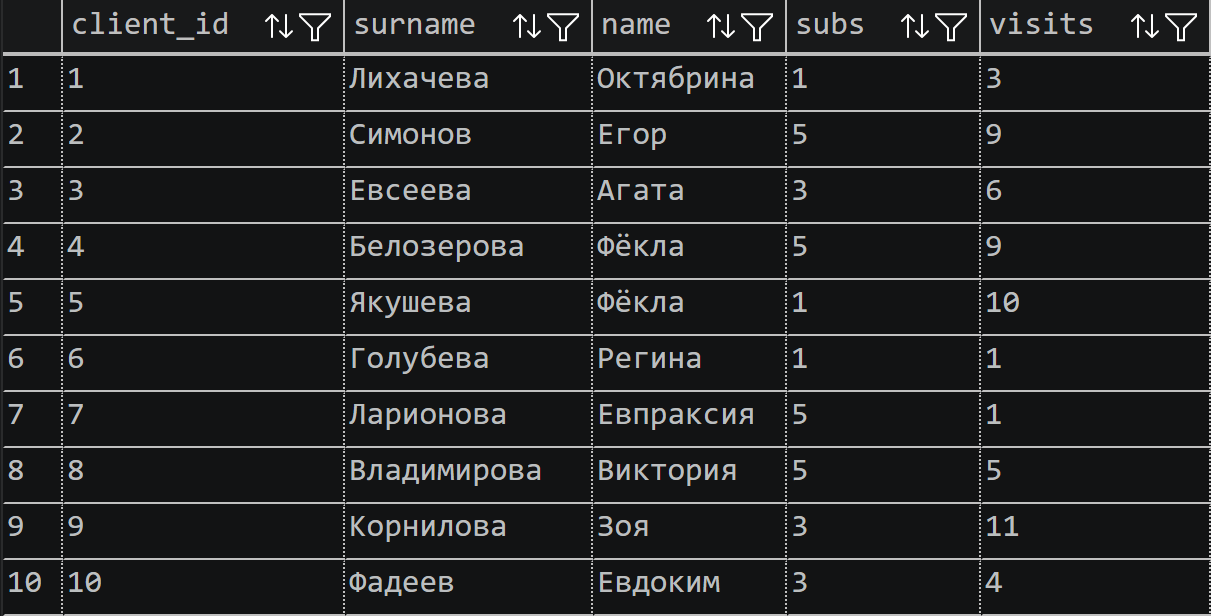
\includegraphics[width=0.8\textwidth]{img/req11.png}
			\caption{Первые 10 записей представления client\_subs\_visits}
			\label{fig:req11}
		\end{figure}
		
		На \cref{fig:view} изображен план выполнения запроса view.sql.
		\begin{figure}[h!]
			\centering
			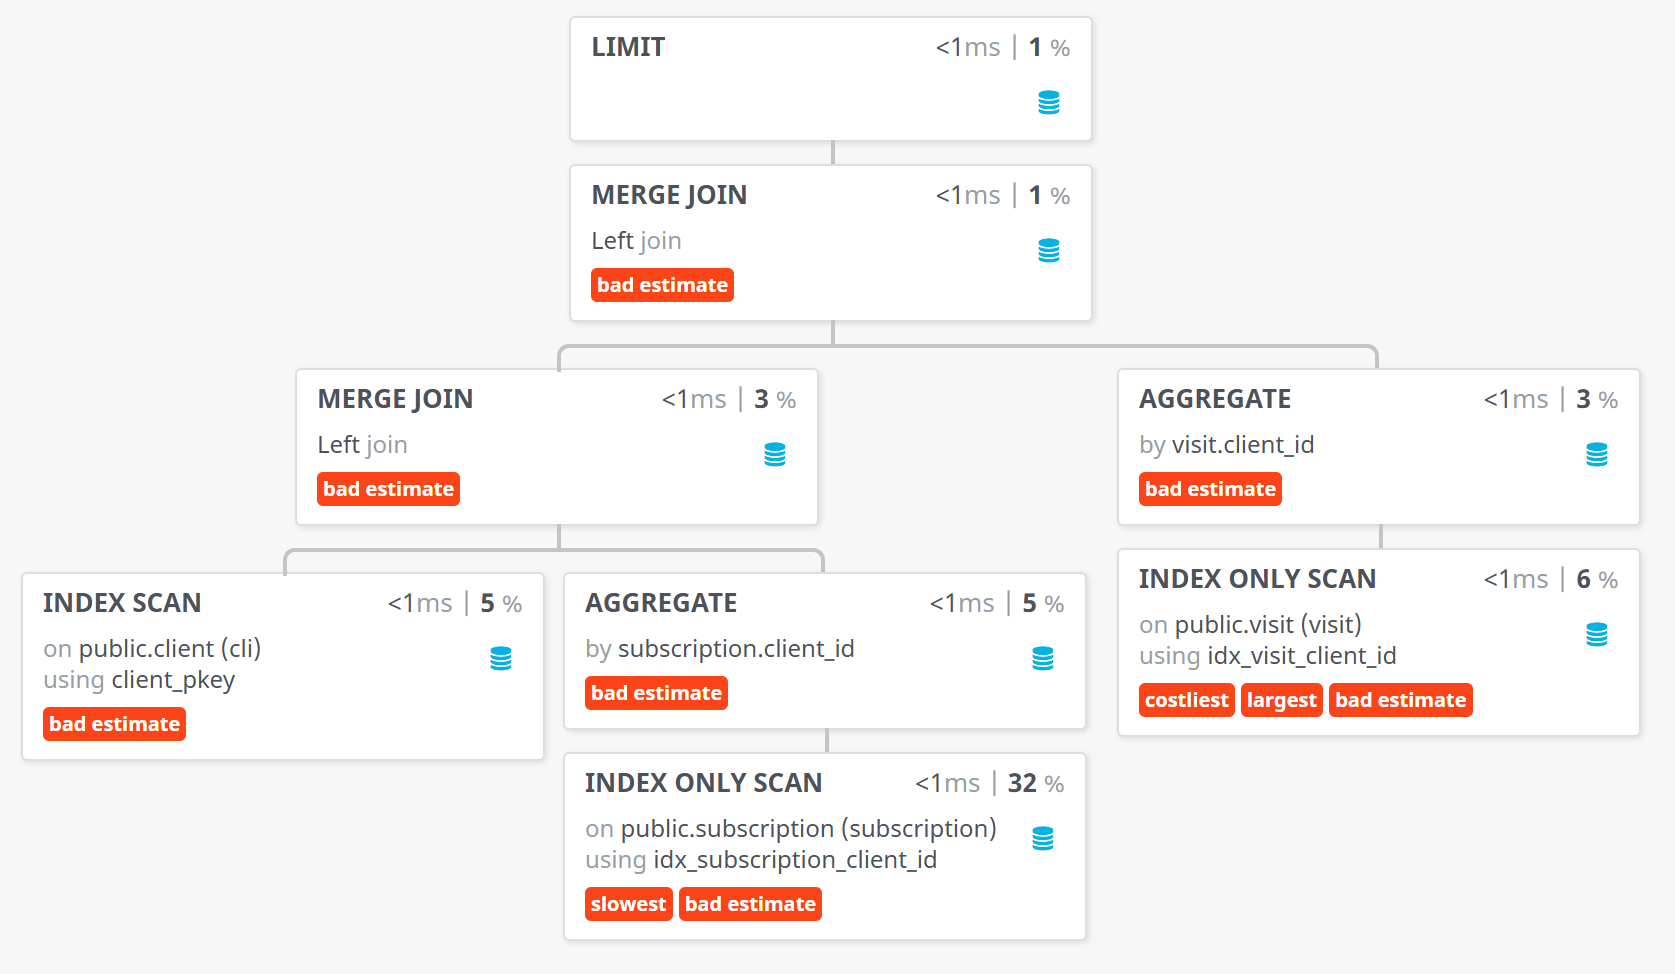
\includegraphics[width=0.8\textwidth]{img/view.png}
			\caption{План выполнения запроса view.sql}
			\label{fig:view}
		\end{figure}
		
		Реляционная формула запроса:
		\begin{equation*}
			\small
			\begin{aligned}
				& \pi_{\text{client\_id, surname, name, subs, visits}} \Bigl( \\
				& \quad \bigl( \text{client} \ltimes_{\text{client.client\_id} = \text{subs.client\_id}} \\
				& \qquad \gamma_{\text{client\_id}; \text{COUNT}(*) \to \text{subs}}(\text{subscription}) \bigr) \\
				& \quad \ltimes_{\text{client.client\_id} = \text{visits.client\_id}} \\
				& \qquad \gamma_{\text{client\_id}; \text{COUNT}(*) \to \text{visits}}(\text{visit}) \Bigr)
			\end{aligned}
		\end{equation*}
		
		Время выполнения запроса --- 3.32~мс.
		
		\subsubsection*{Объяснение плана выполнения запроса}
		\hfill
		
		План запроса выполняет выборку первых 10 записей с использованием левостороннего соединения таблицы клиентов с агрегированными данными по абонементам и визитам, где внешняя таблица сканируется по первичному ключу, а для подсчётов применяются индексы idx\_subscription\_client\_id и idx\_visit\_client\_id в режиме Index Only Scan, после чего результаты объединяются через Merge Join с сортировкой по client\_id.
		
		
	\subsection{Запрос 2}
	\hfill
	
		Вывести идентификаторы, фамилии и имена всех клиентов, которые приобрели более 3 абонементов и совершили более 10 визитов.
		
		Исходный код запроса приведен в \cref{req12}.
		
		\lstinputlisting[firstnumber=1, caption={req2.sql}, label={req12}, language=sql]{../../tasks/01_views/sql/req2.sql}
		
		На \cref{fig:req12} изображен результат запроса 2.
		
		\begin{figure}[h!]
			\centering
			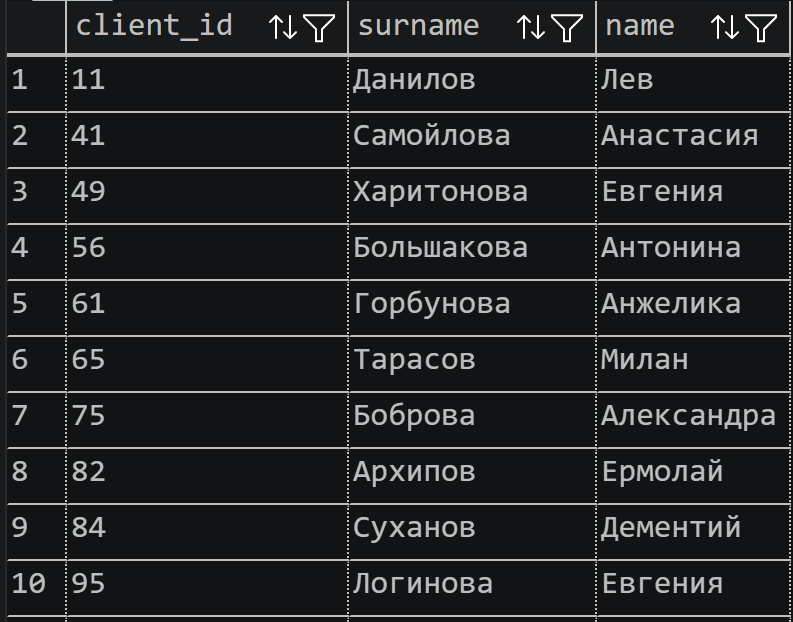
\includegraphics[width=0.8\textwidth]{img/req12.png}
			\caption{Результат запроса 2}
			\label{fig:req12}
		\end{figure}
		
		На \cref{fig:req12explain} изображен план выполнения запроса req12.sql.
		\newpage
		\begin{figure}[h!]
			\centering
			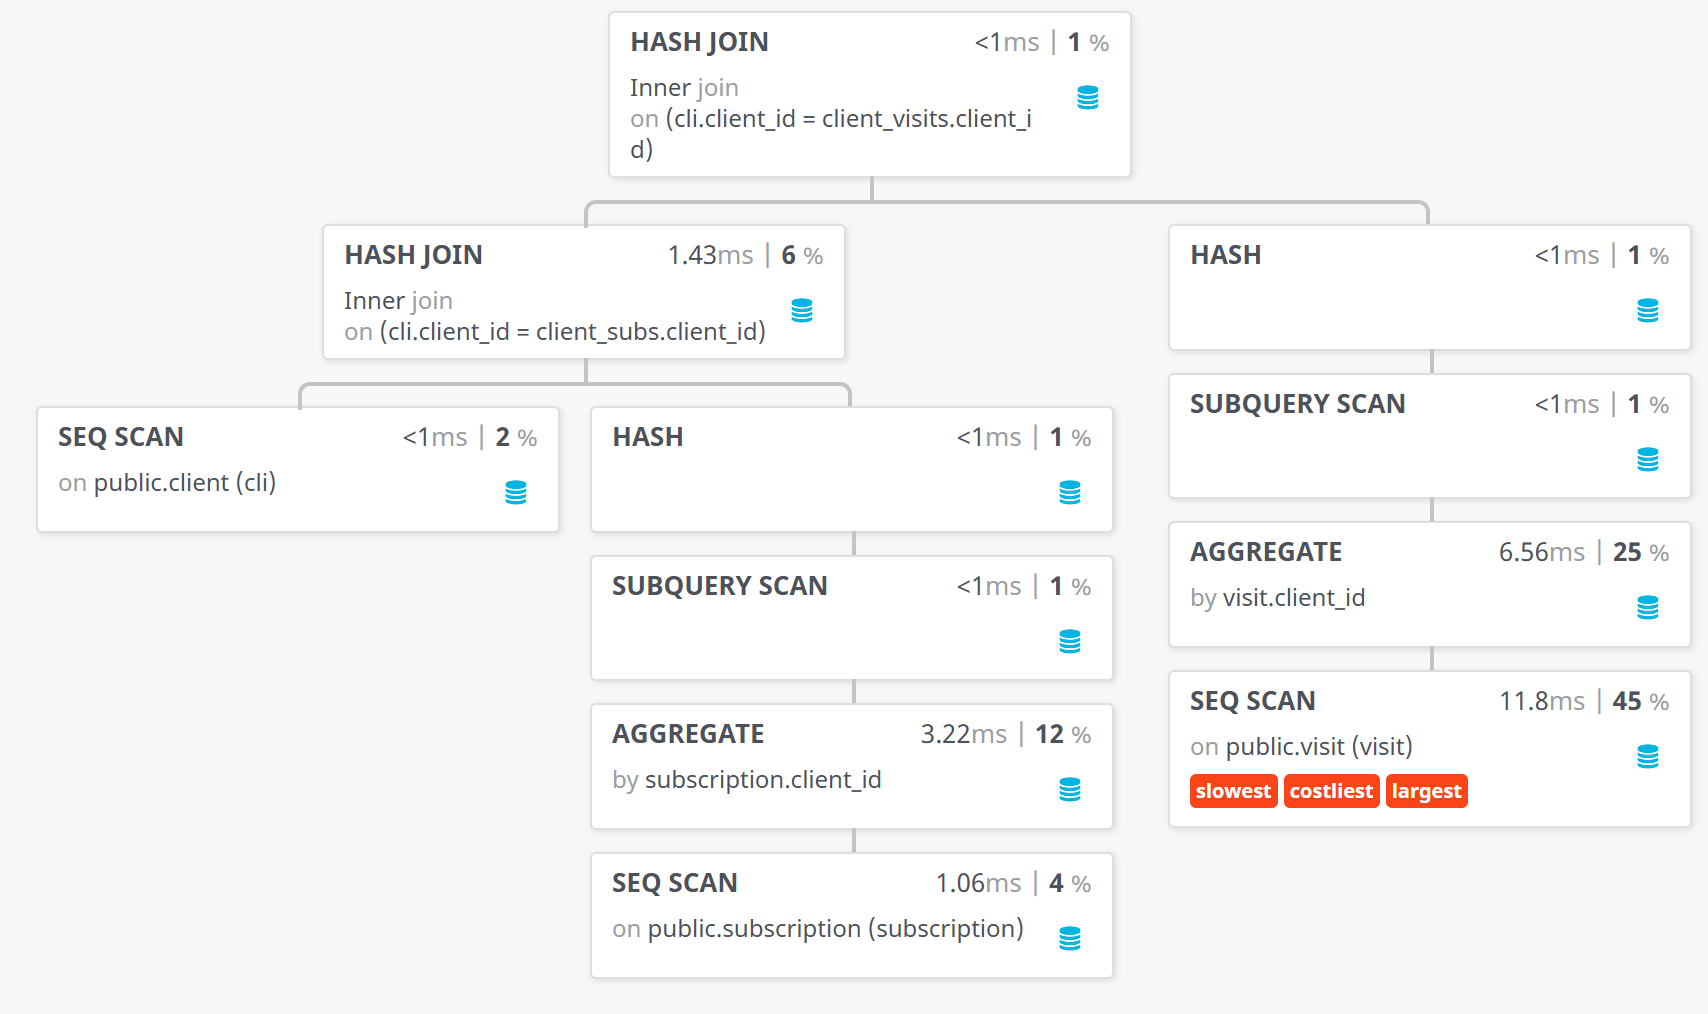
\includegraphics[width=0.8\textwidth]{img/req12explain.png}
			\caption{План выполнения запроса req12.sql}
			\label{fig:req12explain}
		\end{figure}
		
		Реляционная формула запроса:
		\begin{equation*}
			\small
			\begin{aligned}
				& \pi_{\text{client\_id, surname, name}} \Bigl( \\
				& \quad \sigma_{\text{subs} > 3 \wedge \text{visits} > 10} \bigl( \text{client\_subs\_visits} \bigr) \Bigr)
			\end{aligned}
		\end{equation*}
		
		Время выполнения запроса --- 25.97~мс.
		
		\subsubsection*{Объяснение плана выполнения запроса}
		\hfill
		
		План запроса выполняет внутреннее хеш-соединение таблицы client с подзапросом client\_subs, который представляет собой группировку записей subscription по client\_id с фильтром count(*) > 3, после чего полученный результат соединяется внутренним хеш-соединением с подзапросом client\_visits, где записи visit группируются по client\_id с условием count(*) > 10. Все исходные таблицы client, subscription и visit сканируются последовательно, агрегация выполняется хеш-способом, а соединения осуществляются по равенству client\_id.
		
	\subsection{Запрос 3}
	\hfill
	
		Вывести идентификаторы, фамилии и имена всех администраторов, которые заключали договор об аренде хотя бы с одним клиентом, который совершил более 8 визитов.
		
		Исходный код запроса приведен в \cref{req13}.
		
		\lstinputlisting[firstnumber=1, caption={req3.sql}, label={req13}, language=sql]{../../tasks/01_views/sql/req3.sql}
		
		На \cref{fig:req13} изображен результат запроса 3.
		\begin{figure}[h!]
			\centering
			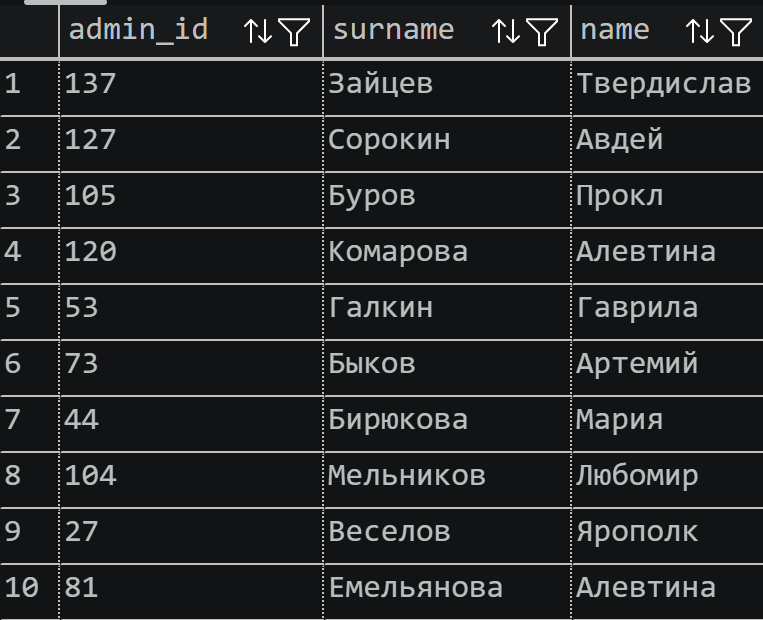
\includegraphics[width=0.8\textwidth]{img/req13.png}
			\caption{Результат запроса 3}
			\label{fig:req13}
		\end{figure}
		
		На \cref{fig:req13explain} изображен план выполнения запроса req13.sql.
		\begin{figure}[h!]
			\centering
			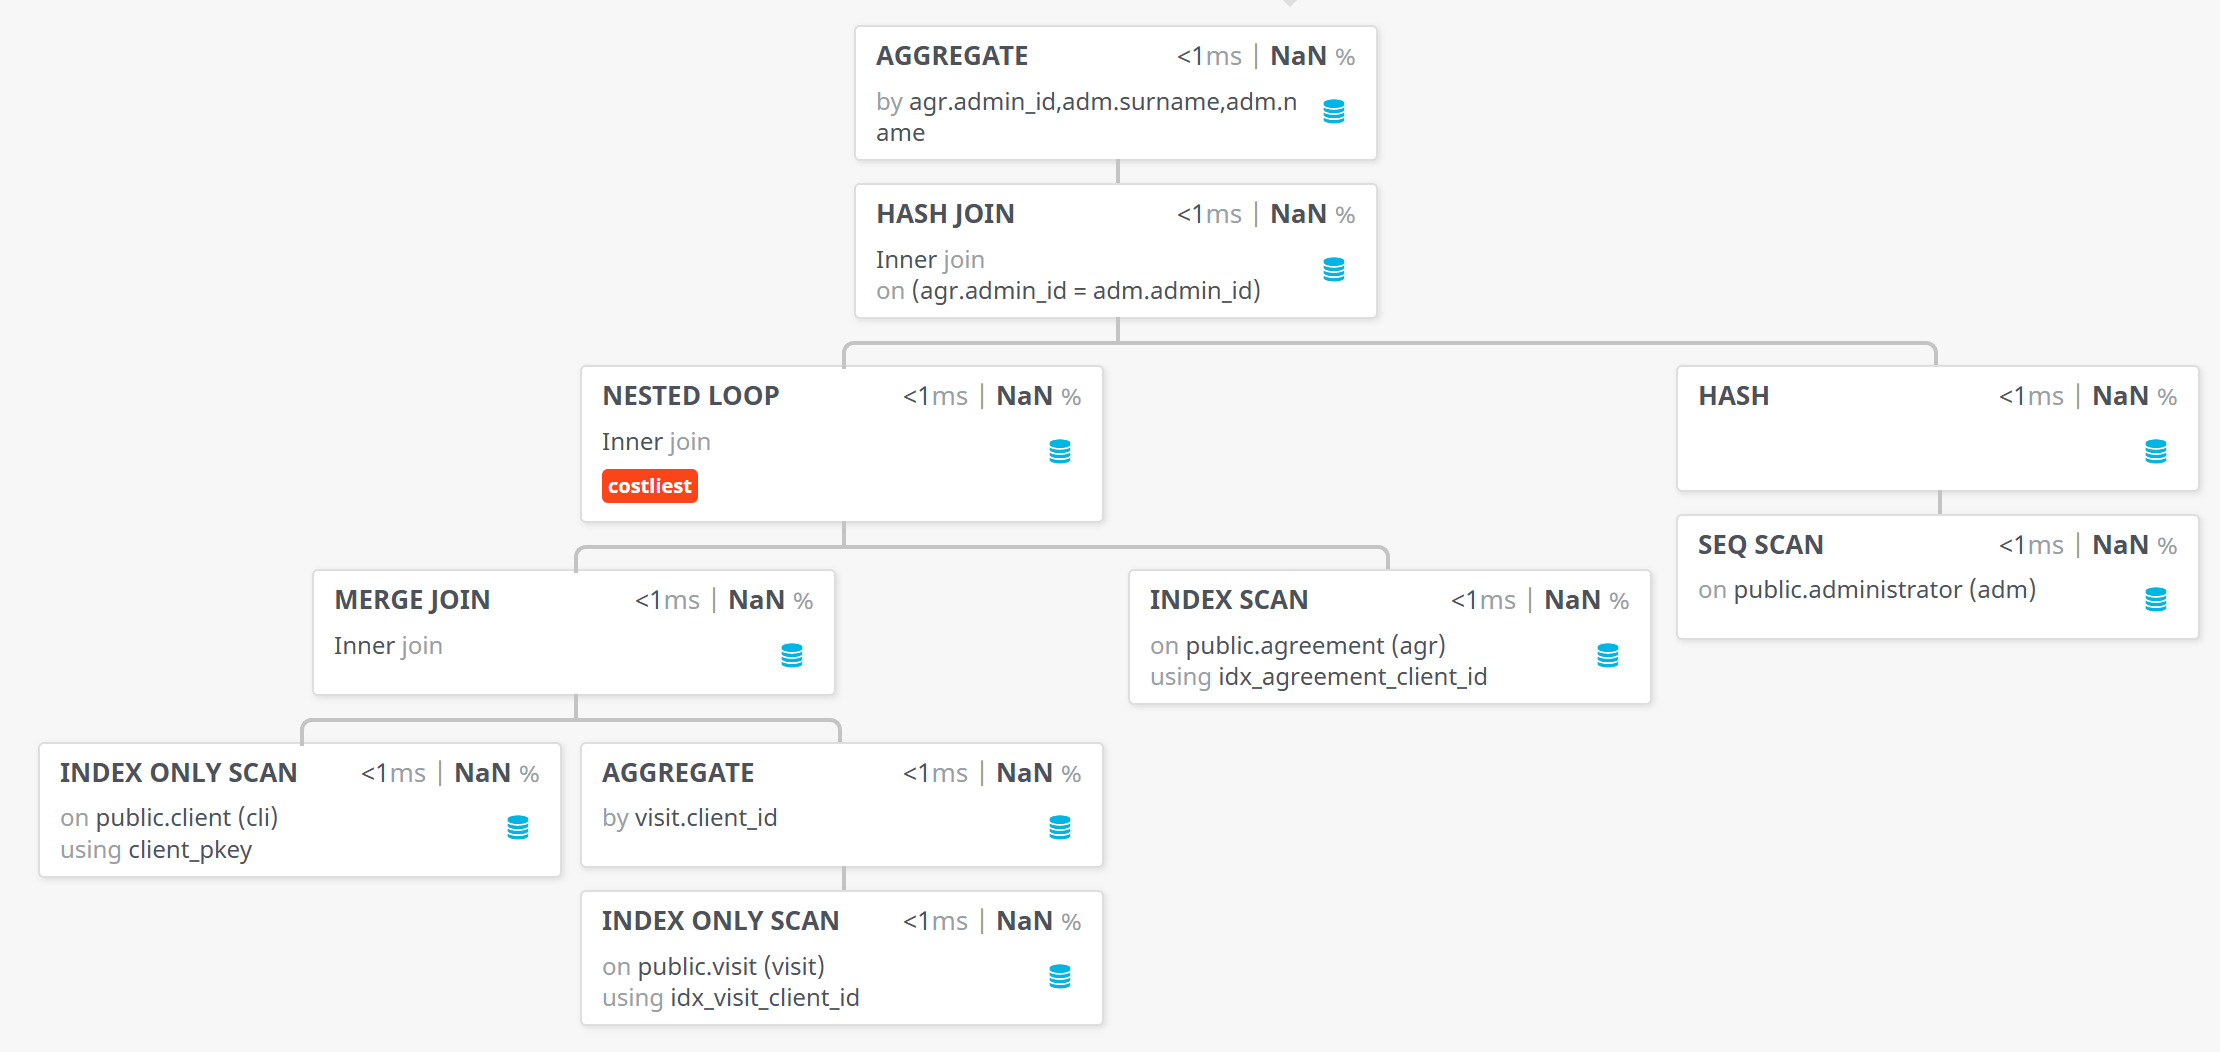
\includegraphics[width=0.8\textwidth]{img/req13explain.png}
			\caption{План выполнения запроса req13.sql}
			\label{fig:req13explain}
		\end{figure}
		
		Реляционная формула запроса:
		\begin{equation*}
			\small
			\begin{aligned}
				& \pi_{\text{administrator.admin\_id}, \text{administrator.surname}, \text{administrator.name}} \Bigl( \\
				& \quad \text{administrator} \bowtie_{\text{administrator.admin\_id} = \text{agreement.admin\_id}} \\
				& \quad \bigl( \text{agreement} \bowtie_{\text{agreement.client\_id} = \text{client\_subs\_visits.client\_id}} \\
				& \qquad \sigma_{\text{visits} > 8}(\text{client\_subs\_visits}) \bigr) \Bigr)
			\end{aligned}
		\end{equation*}
		
		Время выполнения запроса --- 188.43~мс.
		
		\subsubsection*{Объяснение плана выполнения запроса}
		\hfill
		
		Запрос выполняет хешированную агрегацию с группировкой по admin\_id, surname и name, при этом внутренняя часть плана начинается с merge-соединения таблицы client (индексный только-сканирование) с агрегированными по client\_id записями visit (с фильтром count(*) > 8), после чего для каждой пары (cli.client\_id, visit.client\_id) выполняется вложенный цикл с индексным сканированием таблицы agreement по client\_id для получения admin\_id, затем полученный набор admin\_id хеш-соединяется с таблицей administrator (полным сканированием), чтобы добавить surname и name, и наконец внешняя агрегация группирует результат по тем же полям.
	
	
	
	\newpage
	\section{Работа №~2. Триггеры}
	\hfill
	
	
	\section{Работа №~3. Права пользователей}
	\hfill
	
	
	
	\section{Работа №~4. Функции и процедуры}
	\hfill
	
	
	
	\section{Работа №~5. Транзакции}
	\hfill
	
	
	
	\newpage
	\section*{Заключение}
	
	
	
	
	
	
	
	
\end{document}